
\section{Verallgemeinerte NGG-Probleme}
\label{part:verallg-ngg-probl}
Anstelle von $X_{\nu}\subseteq \R^{n_{\nu}}$ betrachten wir $X_{\nu}(x^{-\nu}) \subseteq \R^{n_{\nu}}$ (Ressourcen, die sich alle Spieler teilen müssen).
\subsection{Definition und Beispiele}
\label{sec:defin-und-beisp}
\begin{definition*}
  Gegeben seien $N$ Spieler, Funktionen $f_{\nu}: \R^{n} \lto \R$ für $\nu = 1, \dots, N$ sowie mengenwertige Abbildungen
  \begin{align*}
    X_{\nu}(\cdot): \R^{n_{-\nu}} \rrto\R^{n_{\nu}}. 
  \end{align*}
Unter dem \markdef{verallgemeinerten NGG-Problem} (GNEP) versteht man die Aufgabe, ein $x^{*} = (x^{*, 1}, \dots, x^{*, N}) \in \R^{N}$ zu finden, sodass für alle $\nu = 1, \dots, n$ gilt:
\begin{align}\label{eq:4-1}
&  x^{*, \nu} \in X_{\nu}(x^{*, \nu}) \notag\\
&  f_{\nu}(x^{*, \nu}, x^{*, -\nu}) \leq f_{\nu}(x^{\nu}, x^{*, -\nu}) \quad \forall x^{\nu} \in X_{\nu}(x^{*, -\nu}). 
\end{align}
Ein solcher Vektor $x^{*}$ heißt \markdef{(verallgemeinertes) NGG} oder \markdef{Lösung des GNEP}. Ein Vektor $x \in \R^{n}$ heißt \markdef{zulässig} für das GNEP, wenn $x^{\nu} \in X_{\nu}(x^{-\nu})$ für $\nu = 1, \dots, N$ gilt.  
\end{definition*}
\begin{bemerkung*}
  \begin{enumerate}
  \item Ein $x^{*}$ löst das GNEP genau dann, wenn für jedes $\nu= 1,\dots, N$ die Komponente $x^{*, \nu}$ die Optimierungsaufgabe
    \begin{align*}
      f_{\nu}(x^{\nu}, x^{*, -\nu}) \to \min_{x^{\nu}}, \quad x^{\nu} \in X_{\nu}(x^{*, \nu})
    \end{align*}
ist. 
%\datum{15. Juni 2015}
\item Die mengenwertige Abbildung $X(\cdot): R^{n}\rrto \R^{n}$ sei definiert durch
  \begin{align*}
    X(x) \coloneqq X_{1}(x^{-1}) \times X_{2}(x^{-2}) \times \dots \times X_{n}(x^{-n}). 
  \end{align*}
Dann ist $x \in \R^{n}$ genau dann zulässig für das GNEP, wenn $x \in X(x)$, wenn $x$ also ein Fixpunkt von $X(\cdot)$ ist. 
\item Das NGG-Problem (NEP) kann als Spezialfall des GNEP angesehen werden ($X_\nu(x^{-\nu}) = X_{\nu}$, $X = X_{1} \times \dots \times X_{N}$). 
\item Oft kann $X_{\nu}(x^{-\nu})$ beschrieben werden als
  \begin{align*}
    X_{\nu}(x^{-\nu}) = \set{x^{\nu} \in \R^{n_{\nu}}| g^{\nu}(x^{\nu}, x^{-\nu})\leq 0, \, h^{\nu}(x^{\nu}, x^{-\nu}) = 0}. 
  \end{align*}
  \end{enumerate}
\end{bemerkung*}
\begin{beispiel}\label{ex:4-1} %4.1 
  $N = 2$:
  \begin{align*}
&    x = (x_{1}, x_{2})^{T}\\
&f_{1}(x) = (x_{1} - 1)^{2} \to \min_{x_{1}}, \quad x_{1} + x_{2} \leq 1\\
&f_{2}(x) = (x_{2} - \frac 12)^{2} \to \min_{x_{2}}, \quad x_{1} + x_{2} \leq 1\\
&X_{1}(x_{2}) = \set{x_{1} \in \R| x_{1} \leq 1 - x_{2}} = (- \infty, 1 - x_{2}]\\
&X_{1}(2) = (- \infty, -1]\\
&X_{1}(1) = (- \infty, 0]\\
&X_{1}(-2) = (- \infty, 3]\\
&X_{2}(x_{1}) = \set{x_{2} \in \R| x_{2} \leq 1 - x_{1}} = (- \infty, 1 - x_{1}]\\
&X_{2}(0) = (-\infty, 1]\\
&X_{2}(-1) = (-\infty, 2]
  \end{align*}
  \begin{figure}[h!]
    \centering
    \begin{tikzpicture}
      \draw (-3,0) -- coordinate (x axis mid) (3,0);
    	\draw (0,-3) -- coordinate (y axis mid) (0,3);
    	%ticks
    	\foreach \x in {-3,...,3}
     		\draw (\x,1pt) -- (\x,-3pt)
			node[anchor=north] {\x};
    	\foreach \y in {-3,...,3}
     		\draw (1pt,\y) -- (-3pt,\y) 
     			node[anchor=east] {\y}; 
          \draw[domain=-2:3, variable= \x] plot ({\x},{1 - \x});

          \draw[dotted] (-1, -3) -- (-1, 2);
          \draw[dotted] (-3, -2) -- (3, -2);
    \end{tikzpicture}
    \caption{Visualisierung}
    \label{fig:ex_NEP}
  \end{figure}
Für ausgewählte $x$ soll $X(x)$ berechnet werden (um $x \in X(x)$ zu prüfen).
\begin{align*}
  X(0,1) = X_{1}(1) \times X_{2}(0) = (- \infty, 0] \times (- \infty, 1], 
\end{align*}
also ist $(0, 1) \in X(0, 1)$. 
\begin{align*}
    X(1,1) = X_{1}(1) \times X_{2}(1) = (- \infty, 0] \times (- \infty, 0], 
\end{align*}
also ist $(1, 1) \in X(1, 1)$, alsi ist $(1, 1)$ unzulässig. 
\end{beispiel}
\begin{beispiel} \label{ex:4-2} %4.2
  $N = 2$
  \begin{align*}
    &x = (x_{1} x_{2})^{T}\\
    &f_{1}(x) = (x_{2} + 2)x_{1} \to \min_{x_{1}}, \quad x_{1}^{2} + x_{2}^{2} \leq 1\\
    &f_{2}(x) = (x_{2}^{2} + x_{1}x_{2}) \to \min_{x_{2}}, \quad x_{1} - x_{2}^{2} \leq 0
  \end{align*}
  \begin{align*}
    X_{1}(x_{2}) &=    \begin{cases}
      [- \sqrt{-1 - x_{2}^{2}}, \sqrt{1- x_{2}^{2}}] & \norm{x_{2}}\leq 1\\
      \emptyset & \norm{x_{2}} > 1 \end{cases}\\
    X_{2}(x_{1}) &= \set{x_{2} \in \R| \, x_{2} \geq x_{1}} = [x_{1}, \infty)
  \end{align*}
  \begin{figure}[h!]
    \centering
    \begin{tikzpicture}
      \draw (-2,0) -- coordinate (x axis mid) (2,0);
    	\draw (0,-2) -- coordinate (y axis mid) (0,2);
      \draw (0, 0) circle (1);
    \end{tikzpicture}
    \begin{tikzpicture}
      \draw (-1,0) -- coordinate (x axis mid) (3,0);
    	\draw (0,-1) -- coordinate (y axis mid) (0,3);
      \draw [domain=-0.5:2.5, variable= \x] plot ({\x},{\x});
      \draw[dotted] (2, 2) -- (2, 3);
    \end{tikzpicture}
    \caption{Beispiel}
  \end{figure}
  \begin{align*}
    (0, 0.6) &\in X(0, 0.6) = X_{1}(0.6) \times X_{2}(0) = [-0.8, 0.8] \times [0, \infty)\\
    (0.8, 0.6) &\notin X(0.8, 0.6) = X_{1}(0.6) \times X_{2}(0.8) = [-0.8, 0.8] \times [0.8, \infty)
  \end{align*}
\end{beispiel}
\begin{beispiel}\label{ex:4-3} %4.3
  Oligopolmodell nach Cournot

  \begin{align*}
    f_{\nu}(x_{1}, \dots, x_{N}) &= x_{\nu} \cdot p(x_{1}, \dots, x_{N}) - K_{\nu}(x_{\nu}) \to \max_{x_{\nu}}, \quad x_{\nu} \geq 0, x_{1} + \dots + x_{N} \leq C\\
X_{\nu}(x_{-\nu}) &= \set{x_{\nu} \in \R| 0 \leq x_{\nu}\leq C - \sum_{\eta = 1, \nu \neq \eta}^{N}x_{\eta}}
  \end{align*}
\end{beispiel}
\begin{definition*}
  Für $\nu \in \set{1, \dots, N}$ und $x^{-\nu} \in \R^{-n_{\nu}}$ sei
  \begin{align*}
    S_{\nu}(x^{-\nu}) = \set{x^{\nu} \in X_{\nu}(x^{-\nu})| \, f_{\nu}(x^{\nu}, x^{-\nu}) \leq f_{\nu}(y, x^{-\nu}) \, \forall y^{\nu} \in X_{\nu}(x^{-\nu})}
  \end{align*}
die \markdef{Menge der besten Antworten} des Spielers $\nu$ auf die Strategiekombination $x^{-\nu}$ der Gegenspieler definiert. Die mengenwertige Abbildung $x^{-\nu} \mapsto S_{\nu}(x^{-\nu})$ heißt \markdef{Beste-Antwort-Funktion} des Spielers $\nu$ und die Abbildung $x \mapsto S(x)$ mit
\begin{align*}
  S(x)\coloneqq S_{1}(x^{-1}) \times \dots \times S_{N}(x^{-N})
\end{align*}
\markdef{Beste-Antwort-Funktion} des GNEPs.
\end{definition*}

\begin{satz}\label{thm:4-1} 
 Ein $x^{*} \in \R^{n}$ ist genau dann Lösung des GNEPs, wenn $x^{*}$ Fixpunkt der Abbildung $x \mapsto S(x)$ ist, das heißt, wenn $x^{*} \in S(x^{*})$. 
\end{satz}
\begin{beweis}
   $x^{*}$ ist Lösung des GNEPs $\Leftrightarrow$ $x^{*, \nu} \in X_{\nu}(x^{*, -\nu})$ und \eqref{eq:4-1} erfüllt ist für alle $\nu = 1, \dots, N$ $\Leftrightarrow$ $x^{*, \nu} \in S_{\nu} (x^{*, - \nu})$ für $\nu = 1, \dots, N$ $\Leftrightarrow$ $x^{*} \in S(x^{*})$. 
\end{beweis}
\begin{fortsetzung} Beispiel \ref{ex:4-1}
  Ermittlung von $S_{1}(x_{2})$: Lösung von $(x_{1} - 1)^{2} \to \min_{x_{1}}$ bei $x_{1} \leq 1 - x_{2}$. Ist $x_{2} \leq 0$, dann ist $x_{1} = 1$ zulässig und eindeutige Lösung. Andernfalls ist $x_{1} =  1 - x_{2}$ die eindeutige Lösung.
  \begin{align*}
     S_{1}(x_{2})=
     \begin{cases}
       \set 1, & x_{2} \leq 0\\
       \set{1 - x_{2}}, & x_{2} > 0, 
     \end{cases}
  \end{align*}
Analog erhält man 
  \begin{align*}
     S_{2}(x_{1})=
     \begin{cases}
       \set {\frac 1 2}, & x_{1} \leq \frac 1 2\\
       \set{1 - x_{2}}, & x_{1} > \frac 1 2. 
     \end{cases}. 
  \end{align*}
Achtung, wenn $x_{1} \in S_{1}(x_{2})$ und $x_{2} \in S_{2}(x_{1})$. Lösungsmenge des GNEP ist
\begin{align*}
  \set{t, 1-t \left|\, \frac 1 2 \leq t \leq 1\right.}.
\end{align*}
\end{fortsetzung}
\begin{definition*}
  \begin{itemize}
  \item Ein GNEP heißt \markdef{Spieler-konvex} (\markdef{player convex}), wenn für jeden Spieler $\nu \in \set{1, \dots, N}$ und für jeden Vektor $x^{-\nu} \in \R^{n_{-\nu}}$ die Menge $X_{\nu}(x^{-\nu})$ konvex ist und $f_{\nu}(\cdot, x^{-\nu})$ konvex ist. 
\item Ein GNEP heißt \markdef{GNEP mit gemeinsamen Restriktionen} (\markdef{GNEP with shared/common constraints}), wenn eine nichtleere Menge $X \subseteq \R^{n}$ derart existiert, sodass
  \begin{align*}
    X_{\nu} (x^{-\nu}) = \set{x^{\nu} \in \R^{n}|\, (x^{\nu}, x^{-\nu}) \in X}
  \end{align*}
für alle $\nu = 1, \dots, N$ und alle $x^{-\nu} \in \R^{n_{-\nu}}$. Die Menge $X$ heißt dann \markdef{gemeinsame Strategiemenge}. 
\item Ein GNEP mit gemeinsamen Restriktionen, bei dem $X$ nichtleer und konvex ist und bei dem die Funktionen $f_{\nu}(\cdot, x^{-\nu})$ konvex sind für alle $\nu = 1, \dots, N$ und alle $x^{-\nu} \in \R^{n_{-\nu}}$, heißt \markdef{jointly convex}. 
\end{itemize}
\end{definition*}
\begin{bemerkung*}
  \begin{enumerate}
  \item Ein GNEP, das jointly convex ist, ist auch Spieler-konvex. Die Umkehrung gilt im Allgemeinen nicht. 
    % \datum{18. Juni 2015}
  \item Existieren von $\nu$ unabhängige Funktionen $G$ und $H$, sodass 
    \begin{align*}
      X_{\nu}(x^{-\nu})&= \set{x^{n} \in \R^{n_{\nu}}|\, G(x^{\nu}, x^{-\nu})\leq 0, \, H(x^{\nu}, x^{-\nu})=0}, \\
      (X_{\nu}(x^{-\nu})&= \set{x^{n} \in \R^{n_{\nu}}|\, (x^{\nu}, x^{-\nu}) \in X}, \\
      X &= \set{x^{n} \in \R^{n}|\, G(x) \leq 0, H(x)= 0}), 
    \end{align*}
dann ist auch irgendwas. 
  \end{enumerate}
\end{bemerkung*}
\begin{proposition}\label{prop:4-2}
  Für ein GNEP mit gemeinsamen Restriktionen ist ein Punkt $x \in \R^{n}$ genau dann zulässig, wenn $x \in X$. 
\end{proposition}
\begin{beweis}
  $x$ ist zulässig für das GNEP 
  \begin{align*}
    &\Leftrightarrow x \in X(x) = X_{1}(x^{-1}) \times \dots \times X_{N}(x^{-N})\\
    &\Leftrightarrow \forall \nu \in \set{1, \dots, N}: x^{\nu} \in X_{\nu}(x^{-\nu})\\
    &\Leftrightarrow \forall \nu \in \set{1, \dots, N}: (x^{\nu}, x^{-\nu}) \in \X\\
    &\Leftrightarrow x \in X. 
  \end{align*}
\end{beweis}
\begin{bemerkung*}
  Die Mengen $X$ und $X(x)$ stimmen im Allgemeinen für ein gegebenes $x \in X$ nicht überein. Zum Beispiel sei $X \coloneqq \set{x \in \R^{n}|\, x_{1}^{2} + x_{2}^{2} \leq 1}$ und $\bar x = (0.6 \, 0.6)^{T}$. Dann ist
  \begin{align*}
    X_{1}(\bar x_{2}) = X_{1}(0.6) = [- \sqrt{1 - 0.6^{2}}, \sqrt{1 - 0.6^{2}}] = [-0.8, 0.8] = X_{2}(\bar x_{1}). 
  \end{align*}
Folglich ist $X(x^{2}) = [-0.8, 0.8]^{2}$. 
\begin{figure}[h!]
  \centering

  \caption{Visualisierung}
  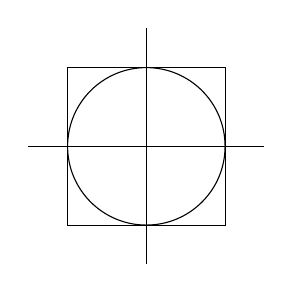
\begin{tikzpicture}
    \draw (-1.5,0) -- coordinate (x axis mid) (1.5,0);
    \draw (0,-1.5) -- coordinate (y axis mid) (0,1.5);
    \draw (-1, -1) rectangle (1, 1);
    \draw (0,0) circle (1);%{\sqrt{2}});
  \end{tikzpicture}
\end{figure}
Also gilt weder $X(\bar x ) \subseteq X$ noch $X \subseteq X(\bar x)$. 
\end{bemerkung*}

\subsection{Umformulierungen von GNEPs}
\label{sec:umform-von-gneps}

\subsubsection{Umformulierungen mithilfe von Nikaido-Isoda-Funktionen}
\label{sec:umform-mith-von}

\begin{align*}
  \Psi(x, y)\coloneqq \sum_{\nu = 1}^{N} \( f_{\nu}(x^{\nu}, x^{-\nu}) - f_{\nu}(y^{\nu}, x^{-\nu}) \)
\end{align*}
\begin{satz}\label{thm:4-3}
  \begin{enumerate}
  \item Ist $x$ zulässig für das GNEP, dann gilt
    \begin{align*}
      \sup_{y \in X(x)} \Psi (x, y) \geq 0. 
    \end{align*}
\item Ein Vektor $x^{*}$ ist genau dann Lösung des GNEP, wenn $x^{*} \in X(x^{*})$ und
    \begin{align*}
      \sup_{y \in X(x^{*})} \Psi (x, y) = 0. 
    \end{align*}
  \end{enumerate}
\end{satz}
\begin{beweis}
  \begin{enumerate}
  \item Da $x$ zulässig ist, gilt $x \in X(x)$ und somit
 \begin{align*}
      \sup_{y \in X(x)} \Psi (x, y) \geq \Psi(x, x) = 0. 
    \end{align*}
\item Sei $x^{*}$ Lösung des GNEP. Dann ist $x^{*}$ zulässig, das heißt $x^{*} \in X(x^{*})$. Sei nun $y \in X(x^{*})$ beliebig gewählt. Wegen $X(x^{*}) = X_{1}(x^{*,-1}) \times \dots \times X_{N}(x^{*,-N})$ ist $y^{\nu} \in X_{\nu}(x^{*, -\nu})$ für alle $\nu = 1, \dots, N$. Da $x^{*}$ Lösung des GNEP ist, folgt
  \begin{align*}
    f_{\nu}(x^{*, \nu}, x^{*, -\nu}) =     f_{\nu}(x^{*}) \leq     f_{\nu}(y^{\nu}, x^{*, -\nu})
  \end{align*}
für alle $\nu = 1, \dots, N$ und somit
\begin{align*}
  \Psi(x^{*}, y) = \sum_{\nu = 1}^{N}\underbrace{ \(f_{\nu} (x^{*}) - f_{\nu}(y^{*}, x^{*, \nu})\)}_{\leq 0} \leq 0. 
\end{align*}
Da $y \in X(x^{*})$ beliebig gewählt wurde, folgt $\sup_{y \in X(x^{*})} \Psi(x^{*}, y) \leq 0$. Zusammen mit der ersten Aussage ergibt sich
\begin{align*}
    \sup_{y \in X(x^{*})} \Psi (x^{*}, y) = 0.
\end{align*}
\vspace{2mm}

Umgekehrt sei $x^{*}$ zulässig und es gelte $\sup_{y \in X(x^{*})} \Psi (x^{*}, y) = 0$. Letzteres impliziert $\Psi(x^{*}, y) \leq 0$ für alle $y \in X(x^{*})$. Seien nun $\nu = \set{1, \dots, N}$ und $x^{\nu} \in X_{\nu} (x^{*, -\nu})$. Wegen $x^{*} \in X(x^{*}) = X_{1}(x^{*,-1}) \times \dots \times X_{N}(x^{*,-N})$ (Zulässigkeit) ist dann $y\coloneqq (x^{*, \nu}, x^{*, -\nu}) \in X(x^{*})$. Daraus folgt
\begin{align*}
  0 \geq \Psi(x^{*}, y) = \sum_{\eta = 1}^{N} \(f_{\eta}(x^{*}) - f_{\eta}(y^{\eta}, x^{*, -\eta})\) = f_{\nu}(x^{*}) - f_{\nu}(x^{\nu}, x^{*, -\nu}), 
\end{align*}
das heißt $f_{\nu}(x^{*}) \leq f_{\nu}(x^{\nu},x^{*, -\nu})$. Da $\nu$ und $x^{\nu}$ beliebig gewählt waren, ist $x^{*}$ eine Lösung des GNEP.
  \end{enumerate}
\end{beweis}
Für den Rest von Abschnitt \ref{sec:umform-mith-von} wird vorausgesetzt, dass das GNEP gemeinsame Restriktionen hat. Für die zugehörige Strategiemenge setzen wir zunächst voraus, dass $X \neq \emptyset$ und $X$ kompakt ist. Des Weiteren wird vorausgesetzt, dass $f_{\nu}: \R^{n} \to \R$ stetig ist für $\nu = 1, \dots, N$. 

Für $x \in X$ ist die Menge $X(x)$ nichtleer, da nach Proposition \ref{prop:4-2} der Vektor $x$ zu $X(x)$ gehört. Außerdem ist $X(x)$ kompakt, da die Mengen 
\begin{align*}
  X_{\nu}(x^{-\nu}) = \set{y^{\nu} \in \R^{n_{\nu}}|\, (y^{\nu}, x^{-\nu}) \in X}
\end{align*}
wegen der Kompaktheit von $X$ beschränkt und abgeschlossen sind. Wir definieren die Funktion $\hat V: X \to \R$ durch
\begin{align*}
  \hat V(x) \coloneqq \max_{y \in X(x)}\Psi(x,y). 
\end{align*}
Diese Funktion ist also wohldefiniert (da das Maximum existiert).
\begin{satz}\label{thm:4-4}
  Die gemeinsame Strategiemenge $X$ sei nichtleer und kompakt und die Funktionen $f_{\nu}$ seien stetig. Dann gilt:
  \begin{enumerate}
  \item $\hat V (x) \geq 0$ für alle $x \in X$. 
  \item $x^{*} \in \R^{n}$ ist genau dann Lösung des GNEPs, wenn $x* \in X$ und $\hat V (x^{*}) = 0$. 
  \end{enumerate}
\end{satz}
\begin{korollar}\label{cor:4-5}
  Unter den Voraussetzungen von Satz \ref{thm:4-4} ist $x^{*}$ genau dann Lösung des GNEP, wenn $x^{*}$ die Optimierungsaufgabe 
  \begin{align*}
    \hat V(x)\to \min_{x \in X}
  \end{align*}
löst und der optimale Zielfunktionswert $\hat V (x^{*}) = 0$ ist. 
\end{korollar}
Nun wird die Voraussetzung der Kompaktheit von $X$ fallen gelassen. Anstelle dessen sei das GNEP nun jointly convex. Zusätzlich sei $X$ abgeschlossen und $f_{1}, \dots, f_{N}$ seien stetig. Wir betrachten nun \markdef{regularisierte Nikaido-Isoda-Funktionen}. Sei $\alpha  > 0$:
\begin{align*}
  \Psi_{\alpha}(x, y)\coloneqq \Psi (x, y) - \frac \alpha 2 \nnorm{x - y}_{2}^{2}. 
\end{align*}
Das Maximierungsproblem
\begin{align*}
  \Psi_{\alpha}(x, y) \to \max_{y \in X(x)}
\end{align*}
besitzt für jedes $x \in X$ eine eindeutige Lösung, die wir mit $\hat y_{\alpha}(x)$ bezeichnen. Weiter sei $\hat V_{\alpha}: X \to \R$ definiert durch
\begin{align*}
  \hat V_{\alpha} (x) \coloneqq \max_{y \in X(x)}\Psi_{\alpha}(x, y). 
\end{align*}
\begin{satz}\label{thm:4-6}
  Sei $\alpha > 0$. Das GNEP sei jointly convex. Die Menge $X$ sei abgeschlossen und $f_{1}, \dots, f_{N}: \R^{n} \to \R$ seien stetig. Dann gilt:
  \begin{enumerate}
  \item  $\hat V_{\alpha} (x) \geq 0$ für alle $x \in X$. 
  \item $x^{*}$ ist genau dann Lösung des GNEP, wenn $x^{*} \in X$ und $\hat V _{\alpha} (x^{*}) = 0$. 
  \end{enumerate}
\end{satz}
\begin{beweis}
  Übung. 
\end{beweis}
%\datum{22. Juni 2015}
\begin{korollar}\label{cor:4-7}
  Unter den Voraussetzungen von Satz \ref{thm:4-6} ist ein $x^{*}$ genau dann Lösung des GNEPs, wenn $x^{*}$ die Optimierungsaufgabe
  \begin{align}\label{eq:4-2}
    \hat V_{\alpha}(x) \lto \min, \quad x \in X 
  \end{align}
löst und der optimale Zielfunktionwert $\hat V_{\alpha} (x^{*}) = 0$ ist. 
\end{korollar}
Im Allgemeinen ist $\hat V_{\alpha}$ nicht differenzierbar. 
\begin{definition*}
  Für ein GNEP mit gemeinsamen Restriktionen heißt ein Vektor $x^{*} \in X$ \markdef{normalisiertes Gleichgewicht}, wenn
  \begin{align*}
    \sup_{y \in X} \Psi(x^{*}, y) = 0. 
  \end{align*}
\end{definition*}
\begin{satz}\label{thm:4-8}
  Gegeben sei ein GNEP mit gemeinsamen Restriktionen. Dann ist jedes normalisierte Gleichgewicht eine Lösung des GNEP. 
\end{satz}
\begin{beweis}
  Übung. 
\end{beweis}
\begin{bemerkung*}
  Die Umkehrung des Satzes \ref{thm:4-8} gilt im Allgemeinen nicht. 
\end{bemerkung*}
\begin{beispiel}\label{ex:4-1}
Betrachte
\begin{align*}
  &f_{1}(x) = (x_{1} - 1)^{2} \to \min_{x_{1}}, \quad x_{1} + x_{2} \leq 1\\
  &f_{2}(x) = \(x_{2} - \frac 1 2\)^{2} \to \min_{x_{2}}, \quad x_{1} + x_{2} \leq 1
\end{align*}
Die zugehörige Nikaido-Isoda-Funktion ist
\begin{align*}
  \Psi(x, y) &= \sum_{\nu = 1}^{2} (f_{\nu}(x^{\nu}, x^{-\nu}) - f_{\nu}(y^{\nu}, x^{-\nu}))\\
  &= (x_{1} - 1)^{2} - (y_{1} - 1)^{2} + \(x_{2} - \frac 1 2\)^{2}  -  \(y_{2} - \frac 1 2\)^{2}.
\end{align*}
Nun gilt:
\begin{align*}
  x^{*} \text{ ist normalisiertes Gleichgewicht }&\iff x^{*} \in X \wedge \sup_{y \in X} \Psi(x^{*}, y) = 0\\
  &\iff x^{*} \text{ löst die Maximierungsaufgabe } \Psi(x^{*}, y) \to \max_{y \in X}
\end{align*}
Im Beispiel bedeutet das, dass $x^{*}$ die Optimierungsaufgabe
\begin{align*}
  (x_{1}^{*}-1)^{2} -   (y_{1}-1)^{2} + \(x_{2}^{*} - \frac 1 2\)^{2} - \(y_{2} - \frac 1 2\)^{2} \to \max_{y}, \quad y_{1} + y_{2} \leq 1\\
   (y_{1}-1)^{2} + \(y_{2} - \frac 1 2\)^{2} \to \min_{y}, \quad y_{1} + y_{2} \leq 1 \\
\implies y_{2}^{2} + y_{2}^{2} - y_{2}  + \frac 14 \to \min, \quad 4y_{2} - 1 = 0\\
\implies y_{1}=\frac 1 4 , y_{2} = \frac 34   
\end{align*}
Also ist $x^{*} = \(\frac 3 4 , \frac 1 4 \)^{T}$ ein normalisiertes Gleichgewicht, es gibt hier kein weiteres normalisiertes Gleichgewicht. $x^{*}$ ist auch Löung des GNEP, aber es gibt unendlich viele davon verschiedene Lösungen des GNEP. 
\end{beispiel}
\begin{bemerkung*}
Multipliziert man die Auszahlungsfunktionen $f_{\nu}$ mit positiven Zahlen $r_{\nu}$, so ändert sich die Menge der Lösungen für dieses GNEP nicht. 
Die Menge der normalisierten Gleichgewichte ändert sich im Allgemeinen aber schon. Modifikation des Beispiels \ref{eq:4-1}:
\begin{align*}
  &f_{1}(x) = (x_{1} - 1)^{2} \to \min_{x_{1}}, \quad x_{1} + x_{2} \leq 1\\
  &f_{2}(x) = 2\(x_{2} - \frac 1 2\)^{2} \to \min_{x_{2}}, \quad x_{1} + x_{2} \leq 1  
\end{align*}
Lösungsmenge des GNEPs:
\begin{align*}
  \set{(t, 1 - t)^{T}| \, t \in \left[0.5, 1\)}
\end{align*}
Das normalisierte Gleichgewicht löst $(y_{1} - 1)^{2} - (y_{2} - 0.5)^{2} \to \min$ bei $y_{1} + y_{2} \leq 1$ und ist $\(\frac 2 3, \frac 13 \)^{T}$. 
\end{bemerkung*} 
Eine Alternative, normalisierte Gleichgewichte einzuführen: 
\begin{definition*}
  $x^{*} \in X$ heißt \markdef{normalisiertes Gleichgewicht} eines GNEP mit gemeinsamer Strategiemenge $X$ und den Auszahlungsfunktionen $f_{1}, \dots, f_{N}$, wenn es $r_{1}> 0, \dots, r_{N}> 0$ gibt, sodass
  \begin{align*}
    \sup_{y \in X} \tilde \Psi(x^{*}, y) = 0, 
  \end{align*}
wobei
\begin{align*}
  \tilde \Psi(x, y) \coloneqq \sum_{\nu = 1}^{N} \(\tilde f_{\nu}(x^{\nu}, x^{-\nu}) - \tilde f_{\nu}(y^{\nu}, x^{-\nu})\) 
\end{align*}
mit $\tilde f_{\nu}\coloneqq r_{\nu}f_{\nu}$. 
\end{definition*}
Sei nun das GNEP wieder jointly convex, $X$ abgeschlossen, $f_{1}, \dots, f_{N}: \R^{n} \to \R$ stetig. Die Optimierungsaufgabe
\begin{align*}
  \Psi_{\alpha}(x, y) \to \max_{y \in X}y. 
\end{align*}
besitzt für jedes $x \in \R^{n}$ eine eindeutige Lösung, die mit $y_{\alpha}(x)$ bezeichnet wird.
\begin{align*}
  V_{\alpha}(x)\coloneqq \max_{y \in X} \Psi_{\alpha}(x, y). 
\end{align*}
\begin{satz}\label{thm:4-9}
  Sei $\alpha > 0$. Das GNEP sei jointly convex, $X$ sei abgeschlossen und $f_{1}, \dots, f_{N}$ seien stetig. Dann gilt
  \begin{enumerate}
  \item $  V_{\alpha}(x)\geq 0$ für alle $x \in X$. 
  \item $x^{*}$ ist genau dann ein normalisiertes Gleichgewicht, wenn $x^{*} \in X$ und $V_{\alpha}(x^{*} = 0$. 
  \end{enumerate}
\end{satz}
\begin{korollar}\label{cor:4-10}
  Unter den Voraussetzungen von Satz \ref{thm:4-9} ist $x^{*}$ genau dann ein normalisiertes Gleichgewicht, wenn $x^{*}$ die Optimierungsaufgabe
  \begin{align*}
    V_{\alpha}(x) \to \min, \quad x \in X
  \end{align*}
löst und der optimale Zielfunktionswert $V_{\alpha}(x^{*}) = 0$ ist. 
\end{korollar}
Im Gegensatz zu $\hat V_{\alpha}$ ist $V_{\alpha}$ stetig differenzierbar, wenn $f_{1}, \dots, f_{N}$ stetig differenzierbar ist.
\begin{satz}\label{thm:4-11}
  Es seien die Voraussetzungen von Satz \ref{thm:4-9} und $f_{1}, \dots, f_{N}$ seien stetig differenzierbar. Dann ist $V_{\alpha}$ stetig differenzierbar mit
  \begin{align*}
    \nabla V_{\alpha}(x) = \left.\nabla_{x}\Psi_{\alpha}(x, y)\right|_{y = y_{\alpha}(x)}. 
  \end{align*}
\end{satz}
Es lässt sich auch eine Umformulierung der Aufgabe, ein normalisiertes Gleichgewicht zu bestimmen, in eine unrestringierte Optimierungsaufgabe angeben.  Für $\beta >\alpha > 0$ und $V_{\alpha\beta}: \R^{n} \to \R$ mit
\begin{align*}
  V_{\alpha\beta}(x) \coloneqq V_{\alpha}(x) - V_{\beta}(x)
\end{align*}
ist $x^{*}$ genau dann ein normalisiertes Gleichgewicht, wenn $x^{*}$ die Optimierungsaufgabe
\begin{align*}
  V_{\alpha\beta} \to \min
\end{align*}
löst und der optimale Zielfunktionswert $V_{\alpha\beta}(x^{*}) = 0$ ist. 
\begin{satz}\label{thm:4-12}
  Sei ein GNEP, das jointly convex ist, mit einer kompakten gemeinsamen Strategiemenge $X$ und mit stetigen Funktionen $f_{1}, \dots, f_{N}$ gegeben. Dann gibt es mindestens ein normalisiertes Gleichgewicht. 
\end{satz}

%%% Local Variables: 
%%% mode: latex
%%% TeX-master: "vorlesung"
%%% End: 
